% !TEX root = main.tex
\zihao{-4}\linespread{1.55}\selectfont
\chapter{模板使用说明}
\section{背景}
作者将要写毕业论文,发现学校并没有研究生毕业论文的\LaTeX 模板,因此根据\href{https://yjsxy.tyust.edu.cn/info/1172/3275.htm}{《太原科技大学研究生学位论文格式的统一要求》}(以下简称《要求》)开发了一个研究生\LaTeX 毕业论文模板。TYUSTthesis(Taiyuan University of Science and Technology thesis)以\myverb{ctexbook}文档类为基础,以基本满足《要求》。但该模板并非官方模板,且不同学院或老师有不同要求,遇到问题请反馈。本模板部分格式参考
\href{https://github.com/tuxify/zzuthesis}{《郑州大学本科毕业设计(论文)和研究生学位论文(含 硕士和博士) LaTeX 模版》}

本项目Github 地址\faGithub :\href{https://github.com/Struggle-best/TYUST_thesis}{ \;\;https://github.com/Struggle-best/TYUST\_thesis}

邮箱:\href{fanchao11429@163.com}{fanchao11429@163.com}

本模板使用\TeX Live2022 + Xe\LaTeX 编译通过。\footnote{软件安装见:\url{http://tug.org/texlive/acquire.html}}
\section{文件结构}
本文档通过\textbf{main.tex} 文件\myverb{\input{ }}命令加入各个章节,\textbf{main.tex}内容如下,各部分按需加入自己文档。

\begin{lstlisting}
\begin{document}
% !TEX root = main.tex
%%%%%%%%%%%%%%%%%%%%%%%%%%%%%%%%%%%%%%%%%%%%%%%%%%
%% classn : 分类号
%% schoolc: 学校代码
%% sclass : 密级
%%%%%%%%%%%%%%%%%%%%%%%%%%%%%%%%%%%%%%%%%%%%%%%%%%
\classn{T P 3 9 1}%必须敲空格实现俩端对齐
\schoolc{1 0 1 0 9}%必须敲空格实现俩端对齐
\sclass{公开}
%%%%%%%%%%%%%%%%%%%%%%%%%%%%%%%%%%%%%%%%%%%%%%%%%%
%% ---------------- 论文封面信息 ----------------- 
%% ctitle     :中文题目
%% etitle     :英文题目
%% authors    :作者姓名
%% supervisor :导师及职称
%% department :培养单位
%% major      :学科专业
%% subdate    :论文提交日期
%% reportdate :论文答辩日期
%% chairman   :答辩委员会主席
%% type       :学术型 or 专业型 (硕士需要)
%%%%%%%%%%%%%%%%%%%%%%%%%%%%%%%%%%%%%%%%%%%%%%%%%%
\ctitle{太原科技大学硕士论文 \LaTeX 模板使用示例}
\etitle{Example of Using the Master's Thesis \LaTeX Template for Taiyuan University of Science and Technology}
\authors{樊超}
\supervisor{王帆 \;副教授}
\department{电子信息工程学院}
\major{控制科学与工程}
\subdate{2024年5月}
\reportdate{2024年5月1日}
\chairman{某某 教授}
\type{学术型}% 硕士论文需要这个信息
%%%%%%%%%%%%%%%%%%%%%%%%%%%%%%%%%%%%%%%%%%%%%%%%%%
%% ------------- 博士论文英文封面信息 ------------- 
%% eauthors     :作者姓名(英)
%% emajor       :学科专业(英)
%% edepartment  :培养单位(英)
%% eschool 		:学校名称(英)
%% esupervisor  :导师及职称(英)
%% edate        :论文提交日期
%%%%%%%%%%%%%%%%%%%%%%%%%%%%%%%%%%%%%%%%%%%%%%%%%%
\eauthors{FAN CHAO}
\emajor{Control Science and Engineering}
\edepartment{School of Electronic Infromation Engineering}
\eschool{Taiyuan University of Science and Technology}
\esupervisor{WANGFAN Associate Professor}
\edate{\today}%\edate{May 14,2024}%封面信息
\maketitle %封面
% ---------- 前文 --------- %
\frontmatter
% !TEX root = main.tex
\begin{cabstract}
中文摘要应简要说明本论文的目的、内容、方法、成果和结
论。要突出论文的创新之处。语言力求精炼、准确。中文摘要,
硕士学位论文要求字数为500 字左右,博士学位论文要求为
1000 字左右。中文摘要下方另起一行,注明本文的关键词(3-8
个)
\ckeywords{TeX/LaTeX;模板说明;关键词;3-8}

\end{cabstract}

\begin{eabstract}

The content of the English abstract should correspond closely to that of the Chinese abstract, while adhering to English grammar, maintaining clarity, and ensuring fluency of expression.
\ekeywords{TeX/LaTeX; Template Description; Keywords; 3-8}
\end{eabstract}


%摘要
\tableofcontents   %目录
%\listoffigures    %插图清单
%\listoftables     %表格清单
%% !TEX root = main.tex
\begin{denotation}[2.5cm]
\item[t] 时间
\item[条目] \zhlipsum[1]
\end{denotation}%主要符号对照表
% ---------- 正文 --------- %
\mainmatter
% !TEX root = main.tex
\zihao{-4}\linespread{1.55}\selectfont
\chapter{模板使用说明}
\section{背景}
作者将要写毕业论文,发现学校并没有研究生毕业论文的\LaTeX 模板,因此根据\href{https://yjsxy.tyust.edu.cn/info/1172/3275.htm}{《太原科技大学研究生学位论文格式的统一要求》}(以下简称《要求》)开发了一个研究生\LaTeX 毕业论文模板。TYUSTthesis(Taiyuan University of Science and Technology thesis)以\myverb{ctexbook}文档类为基础,以基本满足《要求》。但该模板并非官方模板,且不同学院或老师有不同要求,遇到问题请反馈。本模板部分格式参考
\href{https://github.com/tuxify/zzuthesis}{《郑州大学本科毕业设计(论文)和研究生学位论文(含 硕士和博士) LaTeX 模版》}

本项目Github 地址\faGithub :\href{https://github.com/Struggle-best/TYUST_thesis}{ \;\;https://github.com/Struggle-best/TYUST\_thesis}

邮箱:\href{fanchao11429@163.com}{fanchao11429@163.com}

本模板使用\TeX Live2022 + Xe\LaTeX 编译通过。\footnote{软件安装见:\url{http://tug.org/texlive/acquire.html}}
\section{文件结构}
本文档通过\textbf{main.tex} 文件\myverb{\input{ }}命令加入各个章节,\textbf{main.tex}内容如下,各部分按需加入自己文档。

\begin{lstlisting}
\begin{document}
% !TEX root = main.tex
%%%%%%%%%%%%%%%%%%%%%%%%%%%%%%%%%%%%%%%%%%%%%%%%%%
%% classn : 分类号
%% schoolc: 学校代码
%% sclass : 密级
%%%%%%%%%%%%%%%%%%%%%%%%%%%%%%%%%%%%%%%%%%%%%%%%%%
\classn{T P 3 9 1}%必须敲空格实现俩端对齐
\schoolc{1 0 1 0 9}%必须敲空格实现俩端对齐
\sclass{公开}
%%%%%%%%%%%%%%%%%%%%%%%%%%%%%%%%%%%%%%%%%%%%%%%%%%
%% ---------------- 论文封面信息 ----------------- 
%% ctitle     :中文题目
%% etitle     :英文题目
%% authors    :作者姓名
%% supervisor :导师及职称
%% department :培养单位
%% major      :学科专业
%% subdate    :论文提交日期
%% reportdate :论文答辩日期
%% chairman   :答辩委员会主席
%% type       :学术型 or 专业型 (硕士需要)
%%%%%%%%%%%%%%%%%%%%%%%%%%%%%%%%%%%%%%%%%%%%%%%%%%
\ctitle{太原科技大学硕士论文 \LaTeX 模板使用示例}
\etitle{Example of Using the Master's Thesis \LaTeX Template for Taiyuan University of Science and Technology}
\authors{樊超}
\supervisor{王帆 \;副教授}
\department{电子信息工程学院}
\major{控制科学与工程}
\subdate{2024年5月}
\reportdate{2024年5月1日}
\chairman{某某 教授}
\type{学术型}% 硕士论文需要这个信息
%%%%%%%%%%%%%%%%%%%%%%%%%%%%%%%%%%%%%%%%%%%%%%%%%%
%% ------------- 博士论文英文封面信息 ------------- 
%% eauthors     :作者姓名(英)
%% emajor       :学科专业(英)
%% edepartment  :培养单位(英)
%% eschool 		:学校名称(英)
%% esupervisor  :导师及职称(英)
%% edate        :论文提交日期
%%%%%%%%%%%%%%%%%%%%%%%%%%%%%%%%%%%%%%%%%%%%%%%%%%
\eauthors{FAN CHAO}
\emajor{Control Science and Engineering}
\edepartment{School of Electronic Infromation Engineering}
\eschool{Taiyuan University of Science and Technology}
\esupervisor{WANGFAN Associate Professor}
\edate{\today}%\edate{May 14,2024} %封面
\maketitle%封面
% ---------- 前文 --------- %
\frontmatter
% !TEX root = main.tex
\begin{cabstract}
中文摘要应简要说明本论文的目的、内容、方法、成果和结
论。要突出论文的创新之处。语言力求精炼、准确。中文摘要,
硕士学位论文要求字数为500 字左右,博士学位论文要求为
1000 字左右。中文摘要下方另起一行,注明本文的关键词(3-8
个)
\ckeywords{TeX/LaTeX;模板说明;关键词;3-8}

\end{cabstract}

\begin{eabstract}

The content of the English abstract should correspond closely to that of the Chinese abstract, while adhering to English grammar, maintaining clarity, and ensuring fluency of expression.
\ekeywords{TeX/LaTeX; Template Description; Keywords; 3-8}
\end{eabstract}


%摘要
\tableofcontents   %目录
%\listoffigures    %插图清单
%\listoftables     %表格清单
% !TEX root = main.tex
\begin{denotation}[2.5cm]
\item[t] 时间
\item[条目] \zhlipsum[1]
\end{denotation}%主要符号对照表

% ---------- 正文 --------- %
\mainmatter
% !TEX root = main.tex
\zihao{-4}\linespread{1.55}\selectfont
\chapter{模板使用说明}
\section{背景}
作者将要写毕业论文,发现学校并没有研究生毕业论文的\LaTeX 模板,因此根据\href{https://yjsxy.tyust.edu.cn/info/1172/3275.htm}{《太原科技大学研究生学位论文格式的统一要求》}(以下简称《要求》)开发了一个研究生\LaTeX 毕业论文模板。TYUSTthesis(Taiyuan University of Science and Technology thesis)以\myverb{ctexbook}文档类为基础,以基本满足《要求》。但该模板并非官方模板,且不同学院或老师有不同要求,遇到问题请反馈。本模板部分格式参考
\href{https://github.com/tuxify/zzuthesis}{《郑州大学本科毕业设计(论文)和研究生学位论文(含 硕士和博士) LaTeX 模版》}

本项目Github 地址\faGithub :\href{https://github.com/Struggle-best/TYUST_thesis}{ \;\;https://github.com/Struggle-best/TYUST\_thesis}

邮箱:\href{fanchao11429@163.com}{fanchao11429@163.com}

本模板使用\TeX Live2022 + Xe\LaTeX 编译通过。\footnote{软件安装见:\url{http://tug.org/texlive/acquire.html}}
\section{文件结构}
本文档通过\textbf{main.tex} 文件\myverb{\input{ }}命令加入各个章节,\textbf{main.tex}内容如下,各部分按需加入自己文档。

\begin{lstlisting}
\begin{document}
% !TEX root = main.tex
%%%%%%%%%%%%%%%%%%%%%%%%%%%%%%%%%%%%%%%%%%%%%%%%%%
%% classn : 分类号
%% schoolc: 学校代码
%% sclass : 密级
%%%%%%%%%%%%%%%%%%%%%%%%%%%%%%%%%%%%%%%%%%%%%%%%%%
\classn{T P 3 9 1}%必须敲空格实现俩端对齐
\schoolc{1 0 1 0 9}%必须敲空格实现俩端对齐
\sclass{公开}
%%%%%%%%%%%%%%%%%%%%%%%%%%%%%%%%%%%%%%%%%%%%%%%%%%
%% ---------------- 论文封面信息 ----------------- 
%% ctitle     :中文题目
%% etitle     :英文题目
%% authors    :作者姓名
%% supervisor :导师及职称
%% department :培养单位
%% major      :学科专业
%% subdate    :论文提交日期
%% reportdate :论文答辩日期
%% chairman   :答辩委员会主席
%% type       :学术型 or 专业型 (硕士需要)
%%%%%%%%%%%%%%%%%%%%%%%%%%%%%%%%%%%%%%%%%%%%%%%%%%
\ctitle{太原科技大学硕士论文 \LaTeX 模板使用示例}
\etitle{Example of Using the Master's Thesis \LaTeX Template for Taiyuan University of Science and Technology}
\authors{樊超}
\supervisor{王帆 \;副教授}
\department{电子信息工程学院}
\major{控制科学与工程}
\subdate{2024年5月}
\reportdate{2024年5月1日}
\chairman{某某 教授}
\type{学术型}% 硕士论文需要这个信息
%%%%%%%%%%%%%%%%%%%%%%%%%%%%%%%%%%%%%%%%%%%%%%%%%%
%% ------------- 博士论文英文封面信息 ------------- 
%% eauthors     :作者姓名(英)
%% emajor       :学科专业(英)
%% edepartment  :培养单位(英)
%% eschool 		:学校名称(英)
%% esupervisor  :导师及职称(英)
%% edate        :论文提交日期
%%%%%%%%%%%%%%%%%%%%%%%%%%%%%%%%%%%%%%%%%%%%%%%%%%
\eauthors{FAN CHAO}
\emajor{Control Science and Engineering}
\edepartment{School of Electronic Infromation Engineering}
\eschool{Taiyuan University of Science and Technology}
\esupervisor{WANGFAN Associate Professor}
\edate{\today}%\edate{May 14,2024} %封面
\maketitle%封面
% ---------- 前文 --------- %
\frontmatter
% !TEX root = main.tex
\begin{cabstract}
中文摘要应简要说明本论文的目的、内容、方法、成果和结
论。要突出论文的创新之处。语言力求精炼、准确。中文摘要,
硕士学位论文要求字数为500 字左右,博士学位论文要求为
1000 字左右。中文摘要下方另起一行,注明本文的关键词(3-8
个)
\ckeywords{TeX/LaTeX;模板说明;关键词;3-8}

\end{cabstract}

\begin{eabstract}

The content of the English abstract should correspond closely to that of the Chinese abstract, while adhering to English grammar, maintaining clarity, and ensuring fluency of expression.
\ekeywords{TeX/LaTeX; Template Description; Keywords; 3-8}
\end{eabstract}


%摘要
\tableofcontents   %目录
%\listoffigures    %插图清单
%\listoftables     %表格清单
% !TEX root = main.tex
\begin{denotation}[2.5cm]
\item[t] 时间
\item[条目] \zhlipsum[1]
\end{denotation}%主要符号对照表

% ---------- 正文 --------- %
\mainmatter
% !TEX root = main.tex
\zihao{-4}\linespread{1.55}\selectfont
\chapter{模板使用说明}
\section{背景}
作者将要写毕业论文,发现学校并没有研究生毕业论文的\LaTeX 模板,因此根据\href{https://yjsxy.tyust.edu.cn/info/1172/3275.htm}{《太原科技大学研究生学位论文格式的统一要求》}(以下简称《要求》)开发了一个研究生\LaTeX 毕业论文模板。TYUSTthesis(Taiyuan University of Science and Technology thesis)以\myverb{ctexbook}文档类为基础,以基本满足《要求》。但该模板并非官方模板,且不同学院或老师有不同要求,遇到问题请反馈。本模板部分格式参考
\href{https://github.com/tuxify/zzuthesis}{《郑州大学本科毕业设计(论文)和研究生学位论文(含 硕士和博士) LaTeX 模版》}

本项目Github 地址\faGithub :\href{https://github.com/Struggle-best/TYUST_thesis}{ \;\;https://github.com/Struggle-best/TYUST\_thesis}

邮箱:\href{fanchao11429@163.com}{fanchao11429@163.com}

本模板使用\TeX Live2022 + Xe\LaTeX 编译通过。\footnote{软件安装见:\url{http://tug.org/texlive/acquire.html}}
\section{文件结构}
本文档通过\textbf{main.tex} 文件\myverb{\input{ }}命令加入各个章节,\textbf{main.tex}内容如下,各部分按需加入自己文档。

\begin{lstlisting}
\begin{document}
\input{chapter/01coverinfor} %封面
\maketitle%封面
% ---------- 前文 --------- %
\frontmatter
\input{chapter/02abstract}%摘要
\tableofcontents   %目录
%\listoffigures    %插图清单
%\listoftables     %表格清单
\input{chapter/03denotation}%主要符号对照表

% ---------- 正文 --------- %
\mainmatter
\input{chapter/04chapter1}

\bibliography{chapter/13references.bib}%参考文献
% ---------- 附录 --------- %
%\begin{appendix}
%	\input{chapter/10appendices}
%\end{appendix}
\backmatter

\input{chapter/11achievement}%学术成果
\input{chapter/12acknowledgement}%致谢
\end{document}
\end{lstlisting}
\section{文件夹组成}
文件夹组成如下:

\begin{forest}
	pic dir tree,
	where level=0{}{directory,
	},
	[文件夹
	[chapter
	[01coverinfor.tex {\color{gray}论文封面信息},file2
	]
	[02abstract.tex {\color{gray}中英文摘要},file2
	]
	[03denotation.tex {\color{gray}主要符号对照表(可取消)},file2
	]
	[04chapter1.tex {\color{gray}第一章},file2
	]
	[10references.tex {\color{gray}参考文献},file2
	]
	[11appendices.tex {\color{gray}附录(可取消)},file2
	]
	[12achievement.tex {\color{gray}攻读学位期间取得的学术成果},file2
	]
	[13acknowledgement.tex {\color{gray}致谢},file2
	]
	]
	[figure
	[logo {\color{gray}封面logo}
	]
	[page2.png {\color{gray}论文图片存放}, file
	]
	[..., file
	]
	]
	[main.tex {\color{gray}主文件},file2
	]
	[TYUSTthesis.cls {\color{gray}模板格式文件},file2
	]
	]
\end{forest}

\section{参数说明}
本文档结合了硕士与博士学位论文模板,因此在加载TYUSTthesis文档类时有三个可选参数:
\begin{itemize}
	\item master 硕士学位论文(default)
	\item doctor 博士学位论文
	\item encover 博士学位论文英文封面
	\item declare 学位论文原创说明与授权说明
\end{itemize}

例如你想使用硕士论文并包含授权页,可使用下边命令
\begin{lstlisting}
\documentclass[master,declare]{TYUSTthesis}
\end{lstlisting}

你想使用博士论文并包含英文封面,可使用下边命令
\begin{lstlisting}
\documentclass[doctor,encover]{TYUSTthesis}
\end{lstlisting}

你想使用博士论文,包含英文封面,包含授权页,可使用下边命令
\begin{lstlisting}
\documentclass[doctor,encover,declare]{TYUSTthesis}
\end{lstlisting}

\section{预加载宏包}
\begin{table}[hp]
	\renewcommand\arraystretch{1.2}
	\centering  % 显示位置为中间
	\bicaption{预加载宏包}{Preloaded macro package}\label{tab:1}
	\begin{tabular}{ll||ll} %第一列设置宽度为45pt 全为左对齐 没有分割线
		\hline
		宏包 		&说明		    & 宏包 	   & 说明     \\
		\hline 
		geometry  &页边距	     &gbt7714	  &参考文献格式 \\
		float	  &浮动体	     &setspace	  & 设置间距  \\
		mwe 	  &提供示例图片  & graphicx  & 插图       \\
		booktabs  &三线表       & longtable &长表格      \\
		threeparttable&注释表&makecell   &表格内容换行 \\
		multirow  & 合并单元格& calc      & 距离计算   \\
		fontawesome& 字体 &listings    & 代码环境         \\
		mhchem     &化学环境     &chemfig   &化学环境     \\
		amsmath    &数学环境    &amsthm     &数学环境     \\
		amssymb    &数学环境    &amsfonts   &数学环境     \\
		hyperref   & 超链接    &enumitem    &列表         \\
		cleveref   & 引用格式   & algorithm2e & 算法\\
		titletoc   & 目录设置  &setspace     &设置间距    \\
		caption    & 图表标题  &tikz        &画图         \\
		subcaption & 图表标题  &tcolorbox   & 彩色盒子   \\
		bicaption &  图表标题   & xparse    &  边注       \\
		marginnote&  边注      &forest      &             \\
		zhlipsum    &            &needspace  &               \\
        lipsum     &    & &\\
		\hline
	\end{tabular}
\end{table}


\bibliography{chapter/13references.bib}%参考文献
% ---------- 附录 --------- %
%\begin{appendix}
%	% !TEX root = main.tex
\section{论文无需附录去掉该部分}
嘻嘻
\section{一些测试}
\subsection{图}
\begin{figure}[H]
	\centering
	\includegraphics[scale=0.5]{example-image}
%	\caption{长标题测试。这是个很长很长很长很长很长很长很长很长很长很长很长很长很长很长很长很长很长很长很长的标题}
\end{figure}
\subsection{表格}
\begin{table}[H]
	\centering
	\caption{三线表}
	\setlength{\tabcolsep}{10mm}{
		\begin{tabular}{cc} 
			\toprule 
			输入& 输出                           \\ 
			\midrule 
			$ SB_{0} $\qquad I0.0& $ D_{1} $灯 \qquad Q0.0    \\ 
			$ SB_{1} $\qquad I0.1& $ D_{2} $灯 \qquad Q0.1    \\ 
			\bottomrule 
		\end{tabular}
	}
\end{table}
\subsection{数学公式}
\[ f(x) = \int_{-\infty}^\infty  \hat f(x)\xi\,e^{2 \pi i \xi x}  \,\mathrm{d}\xi  \]
\begin{equation} 
	\begin{bmatrix}
		z_{1}\\
		z_{2}\\
		\vdots\\
		z_{n}
	\end{bmatrix}
	=\begin{bmatrix}
		1 & x_{1}  &x_{1}^{2}  \\
		1& x_{2} & x_{2}^{2} \\
		\vdots & \vdots & \vdots\\
		1 & x_{n} & x_{3}^{2}
	\end{bmatrix}
	\begin{bmatrix}
		a_{1} \\
		a_{2} \\
		a_{3} 
	\end{bmatrix}
\end{equation}

\begin{equation}
	y_{n}=y_{max} \times e^{\left (-\frac{(x_{n}-x_{max})^{2}}{Q} \right )}
\end{equation}
\section{冒泡排序算法}
君子曰:学不可以已。青,取之于蓝,而青于蓝;冰,水为之,而寒于水。
木直中绳。(车柔)以为轮,其曲中规。虽有槁暴,不复挺者,(车柔)使之然也。故木
受绳则直, 金就砺则利,君子博学而日参省乎己,则知明而行无过矣。吾尝终日而思矣
,  不如须臾之所学也;吾尝(足齐)而望矣,不如登高之博见也。登高而招,臂非加长
也,  而见者远;  顺风而呼,  声非加疾也,而闻者彰。假舆马者,非利足也,而致千
里;假舟楫者,非能水也,而绝江河,  君子生非异也,善假于物也。积土成山,风雨兴
焉;积水成渊,蛟龙生焉;积善成德,而神明自得,圣心备焉。故不积跬步,无以至千里
;不积小流,无以成江海。骐骥一跃,不能十步;驽马十驾,功在不舍。锲而舍之,朽木
不折;  锲而不舍,金石可镂。蚓无爪牙之利,筋骨之强,上食埃土,下饮黄泉,用心一
也。蟹六跪而二螯,非蛇鳝之穴无可寄托者,用心躁也。——荀况
\begin{lstlisting}[language=Java]
	/*冒泡排序算法*/ 
	public static void bubble_sort(int[] arr) {
		int i, j, temp, len = arr.length;
		for (i = 0; i < len - 1; i++)
		for (j = 0; j < len - 1 - i; j++) 
		if (arr[j] > arr[j + 1]) {
			temp = arr[j];
			arr[j] = arr[j + 1];
			arr[j + 1] = temp;
		}
	}
\end{lstlisting}
%\end{appendix}
\backmatter

% !TEX root = main.tex
\begin{achievement}
\begin{enumerate}[font=\heiti]
\item[一、] {\heiti 学术论文}
\begin{enumerate}[{[}1{]},parsep=-.1cm]
	\item {\heiti 章安良}, 刘尉悦, 蒋志迪, 费景臣. 基于声表面波技术的数字微流体微加热器研究[J]. 微纳电子技术, 2008, 45(7): 411-414.(对应论文第3章)
	\item {\heiti Yan Liu}, Chenxiang Lin, Hanying Li, Hao Yan. Protein nanoarrays: Aptamer-directed self-assembly of protein arrays on a DNA nanostructure[J]. Angew Chem Int Ed, 2005, 44(25): 4333-4338.(SCI一区, 对应论文第4章)
\end{enumerate}

\item[二、] {\heiti 国家发明专利}
\begin{enumerate}[{[}1{]},parsep=-.1cm]
	\item {\heiti XXX}, XXX, XXX, XXX. 专利题目. 专利类型. 授权公告号, 授权公告日
	\item XXX, XXX, XXX, XXX. 专利题目. 专利类型. 申请公布号, 申请公布日.
	\item {\heiti 张凯军}, 赵永杰, 陈朝岗. 轨道火车及高速轨道火车紧急安全制动辅助装置. 实用新型专利. CN201220158825.2. 2012-04-05.
\end{enumerate}

\item[三、] {\heiti 科研项目}
\begin{enumerate}[{[}1{]},parsep=-.1cm]
	\item 项目类型, 项目名称, 项目编号, 资助单位, 起止时间, 主持/参与.
\end{enumerate}

\item[四、] {\heiti 其他}
\begin{enumerate}[{[}1{]},parsep=-.1cm]
	\item 
\end{enumerate}

\end{enumerate}
\end{achievement}%学术成果
% !TEX root = main.tex
\begin{ack}
\zhlipsum[1-2]



\end{ack}%致谢
\end{document}
\end{lstlisting}
\section{文件夹组成}
文件夹组成如下:

\begin{forest}
	pic dir tree,
	where level=0{}{directory,
	},
	[文件夹
	[chapter
	[01coverinfor.tex {\color{gray}论文封面信息},file2
	]
	[02abstract.tex {\color{gray}中英文摘要},file2
	]
	[03denotation.tex {\color{gray}主要符号对照表(可取消)},file2
	]
	[04chapter1.tex {\color{gray}第一章},file2
	]
	[10references.tex {\color{gray}参考文献},file2
	]
	[11appendices.tex {\color{gray}附录(可取消)},file2
	]
	[12achievement.tex {\color{gray}攻读学位期间取得的学术成果},file2
	]
	[13acknowledgement.tex {\color{gray}致谢},file2
	]
	]
	[figure
	[logo {\color{gray}封面logo}
	]
	[page2.png {\color{gray}论文图片存放}, file
	]
	[..., file
	]
	]
	[main.tex {\color{gray}主文件},file2
	]
	[TYUSTthesis.cls {\color{gray}模板格式文件},file2
	]
	]
\end{forest}

\section{参数说明}
本文档结合了硕士与博士学位论文模板,因此在加载TYUSTthesis文档类时有三个可选参数:
\begin{itemize}
	\item master 硕士学位论文(default)
	\item doctor 博士学位论文
	\item encover 博士学位论文英文封面
	\item declare 学位论文原创说明与授权说明
\end{itemize}

例如你想使用硕士论文并包含授权页,可使用下边命令
\begin{lstlisting}
\documentclass[master,declare]{TYUSTthesis}
\end{lstlisting}

你想使用博士论文并包含英文封面,可使用下边命令
\begin{lstlisting}
\documentclass[doctor,encover]{TYUSTthesis}
\end{lstlisting}

你想使用博士论文,包含英文封面,包含授权页,可使用下边命令
\begin{lstlisting}
\documentclass[doctor,encover,declare]{TYUSTthesis}
\end{lstlisting}

\section{预加载宏包}
\begin{table}[hp]
	\renewcommand\arraystretch{1.2}
	\centering  % 显示位置为中间
	\bicaption{预加载宏包}{Preloaded macro package}\label{tab:1}
	\begin{tabular}{ll||ll} %第一列设置宽度为45pt 全为左对齐 没有分割线
		\hline
		宏包 		&说明		    & 宏包 	   & 说明     \\
		\hline 
		geometry  &页边距	     &gbt7714	  &参考文献格式 \\
		float	  &浮动体	     &setspace	  & 设置间距  \\
		mwe 	  &提供示例图片  & graphicx  & 插图       \\
		booktabs  &三线表       & longtable &长表格      \\
		threeparttable&注释表&makecell   &表格内容换行 \\
		multirow  & 合并单元格& calc      & 距离计算   \\
		fontawesome& 字体 &listings    & 代码环境         \\
		mhchem     &化学环境     &chemfig   &化学环境     \\
		amsmath    &数学环境    &amsthm     &数学环境     \\
		amssymb    &数学环境    &amsfonts   &数学环境     \\
		hyperref   & 超链接    &enumitem    &列表         \\
		cleveref   & 引用格式   & algorithm2e & 算法\\
		titletoc   & 目录设置  &setspace     &设置间距    \\
		caption    & 图表标题  &tikz        &画图         \\
		subcaption & 图表标题  &tcolorbox   & 彩色盒子   \\
		bicaption &  图表标题   & xparse    &  边注       \\
		marginnote&  边注      &forest      &             \\
		zhlipsum    &            &needspace  &               \\
        lipsum     &    & &\\
		\hline
	\end{tabular}
\end{table}


\bibliography{chapter/13references.bib}%参考文献
% ---------- 附录 --------- %
%\begin{appendix}
%	% !TEX root = main.tex
\section{论文无需附录去掉该部分}
嘻嘻
\section{一些测试}
\subsection{图}
\begin{figure}[H]
	\centering
	\includegraphics[scale=0.5]{example-image}
%	\caption{长标题测试。这是个很长很长很长很长很长很长很长很长很长很长很长很长很长很长很长很长很长很长很长的标题}
\end{figure}
\subsection{表格}
\begin{table}[H]
	\centering
	\caption{三线表}
	\setlength{\tabcolsep}{10mm}{
		\begin{tabular}{cc} 
			\toprule 
			输入& 输出                           \\ 
			\midrule 
			$ SB_{0} $\qquad I0.0& $ D_{1} $灯 \qquad Q0.0    \\ 
			$ SB_{1} $\qquad I0.1& $ D_{2} $灯 \qquad Q0.1    \\ 
			\bottomrule 
		\end{tabular}
	}
\end{table}
\subsection{数学公式}
\[ f(x) = \int_{-\infty}^\infty  \hat f(x)\xi\,e^{2 \pi i \xi x}  \,\mathrm{d}\xi  \]
\begin{equation} 
	\begin{bmatrix}
		z_{1}\\
		z_{2}\\
		\vdots\\
		z_{n}
	\end{bmatrix}
	=\begin{bmatrix}
		1 & x_{1}  &x_{1}^{2}  \\
		1& x_{2} & x_{2}^{2} \\
		\vdots & \vdots & \vdots\\
		1 & x_{n} & x_{3}^{2}
	\end{bmatrix}
	\begin{bmatrix}
		a_{1} \\
		a_{2} \\
		a_{3} 
	\end{bmatrix}
\end{equation}

\begin{equation}
	y_{n}=y_{max} \times e^{\left (-\frac{(x_{n}-x_{max})^{2}}{Q} \right )}
\end{equation}
\section{冒泡排序算法}
君子曰:学不可以已。青,取之于蓝,而青于蓝;冰,水为之,而寒于水。
木直中绳。(车柔)以为轮,其曲中规。虽有槁暴,不复挺者,(车柔)使之然也。故木
受绳则直, 金就砺则利,君子博学而日参省乎己,则知明而行无过矣。吾尝终日而思矣
,  不如须臾之所学也;吾尝(足齐)而望矣,不如登高之博见也。登高而招,臂非加长
也,  而见者远;  顺风而呼,  声非加疾也,而闻者彰。假舆马者,非利足也,而致千
里;假舟楫者,非能水也,而绝江河,  君子生非异也,善假于物也。积土成山,风雨兴
焉;积水成渊,蛟龙生焉;积善成德,而神明自得,圣心备焉。故不积跬步,无以至千里
;不积小流,无以成江海。骐骥一跃,不能十步;驽马十驾,功在不舍。锲而舍之,朽木
不折;  锲而不舍,金石可镂。蚓无爪牙之利,筋骨之强,上食埃土,下饮黄泉,用心一
也。蟹六跪而二螯,非蛇鳝之穴无可寄托者,用心躁也。——荀况
\begin{lstlisting}[language=Java]
	/*冒泡排序算法*/ 
	public static void bubble_sort(int[] arr) {
		int i, j, temp, len = arr.length;
		for (i = 0; i < len - 1; i++)
		for (j = 0; j < len - 1 - i; j++) 
		if (arr[j] > arr[j + 1]) {
			temp = arr[j];
			arr[j] = arr[j + 1];
			arr[j + 1] = temp;
		}
	}
\end{lstlisting}
%\end{appendix}
\backmatter

% !TEX root = main.tex
\begin{achievement}
\begin{enumerate}[font=\heiti]
\item[一、] {\heiti 学术论文}
\begin{enumerate}[{[}1{]},parsep=-.1cm]
	\item {\heiti 章安良}, 刘尉悦, 蒋志迪, 费景臣. 基于声表面波技术的数字微流体微加热器研究[J]. 微纳电子技术, 2008, 45(7): 411-414.(对应论文第3章)
	\item {\heiti Yan Liu}, Chenxiang Lin, Hanying Li, Hao Yan. Protein nanoarrays: Aptamer-directed self-assembly of protein arrays on a DNA nanostructure[J]. Angew Chem Int Ed, 2005, 44(25): 4333-4338.(SCI一区, 对应论文第4章)
\end{enumerate}

\item[二、] {\heiti 国家发明专利}
\begin{enumerate}[{[}1{]},parsep=-.1cm]
	\item {\heiti XXX}, XXX, XXX, XXX. 专利题目. 专利类型. 授权公告号, 授权公告日
	\item XXX, XXX, XXX, XXX. 专利题目. 专利类型. 申请公布号, 申请公布日.
	\item {\heiti 张凯军}, 赵永杰, 陈朝岗. 轨道火车及高速轨道火车紧急安全制动辅助装置. 实用新型专利. CN201220158825.2. 2012-04-05.
\end{enumerate}

\item[三、] {\heiti 科研项目}
\begin{enumerate}[{[}1{]},parsep=-.1cm]
	\item 项目类型, 项目名称, 项目编号, 资助单位, 起止时间, 主持/参与.
\end{enumerate}

\item[四、] {\heiti 其他}
\begin{enumerate}[{[}1{]},parsep=-.1cm]
	\item 
\end{enumerate}

\end{enumerate}
\end{achievement}%学术成果
% !TEX root = main.tex
\begin{ack}
\zhlipsum[1-2]



\end{ack}%致谢
\end{document}
\end{lstlisting}
\section{文件夹组成}
文件夹组成如下:

\begin{forest}
	pic dir tree,
	where level=0{}{directory,
	},
	[文件夹
	[chapter
	[01coverinfor.tex {\color{gray}论文封面信息},file2
	]
	[02abstract.tex {\color{gray}中英文摘要},file2
	]
	[03denotation.tex {\color{gray}主要符号对照表(可取消)},file2
	]
	[04chapter1.tex {\color{gray}第一章},file2
	]
	[10references.tex {\color{gray}参考文献},file2
	]
	[11appendices.tex {\color{gray}附录(可取消)},file2
	]
	[12achievement.tex {\color{gray}攻读学位期间取得的学术成果},file2
	]
	[13acknowledgement.tex {\color{gray}致谢},file2
	]
	]
	[figure
	[logo {\color{gray}封面logo}
	]
	[page2.png {\color{gray}论文图片存放}, file
	]
	[..., file
	]
	]
	[main.tex {\color{gray}主文件},file2
	]
	[TYUSTthesis.cls {\color{gray}模板格式文件},file2
	]
	]
\end{forest}

\section{参数说明}
本文档结合了硕士与博士学位论文模板,因此在加载TYUSTthesis文档类时有三个可选参数:
\begin{itemize}
	\item master 硕士学位论文(default)
	\item doctor 博士学位论文
	\item encover 博士学位论文英文封面
	\item declare 学位论文原创说明与授权说明
\end{itemize}

例如你想使用硕士论文并包含授权页,可使用下边命令
\begin{lstlisting}
\documentclass[master,declare]{TYUSTthesis}
\end{lstlisting}

你想使用博士论文并包含英文封面,可使用下边命令
\begin{lstlisting}
\documentclass[doctor,encover]{TYUSTthesis}
\end{lstlisting}

你想使用博士论文,包含英文封面,包含授权页,可使用下边命令
\begin{lstlisting}
\documentclass[doctor,encover,declare]{TYUSTthesis}
\end{lstlisting}

\section{预加载宏包}
\begin{table}[hp]
	\renewcommand\arraystretch{1.2}
	\centering  % 显示位置为中间
	\bicaption{预加载宏包}{Preloaded macro package}\label{tab:1}
	\begin{tabular}{ll||ll} %第一列设置宽度为45pt 全为左对齐 没有分割线
		\hline
		宏包 		&说明		    & 宏包 	   & 说明     \\
		\hline 
		geometry  &页边距	     &gbt7714	  &参考文献格式 \\
		float	  &浮动体	     &setspace	  & 设置间距  \\
		mwe 	  &提供示例图片  & graphicx  & 插图       \\
		booktabs  &三线表       & longtable &长表格      \\
		threeparttable&注释表&makecell   &表格内容换行 \\
		multirow  & 合并单元格& calc      & 距离计算   \\
		fontawesome& 字体 &listings    & 代码环境         \\
		mhchem     &化学环境     &chemfig   &化学环境     \\
		amsmath    &数学环境    &amsthm     &数学环境     \\
		amssymb    &数学环境    &amsfonts   &数学环境     \\
		hyperref   & 超链接    &enumitem    &列表         \\
		cleveref   & 引用格式   & algorithm2e & 算法\\
		titletoc   & 目录设置  &setspace     &设置间距    \\
		caption    & 图表标题  &tikz        &画图         \\
		subcaption & 图表标题  &tcolorbox   & 彩色盒子   \\
		bicaption &  图表标题   & xparse    &  边注       \\
		marginnote&  边注      &forest      &             \\
		zhlipsum    &            &needspace  &               \\
        lipsum     &    & &\\
		\hline
	\end{tabular}
\end{table}

% !TEX root = main.tex
\zihao{-4}\linespread{1.55}\selectfont
\chapter{模板使用Q\&A}
\begin{mybox}{当我用 \LaTeX 写了论文以后,导师要求用 word 怎么办?}
说服你导师或者顺从你导师。或者给你导师看word,打印时用\LaTeX,毕竟\LaTeX 排版效果确实比 word 好。
\end{mybox}
\begin{mybox}{知网查重必须要求word怎么办?}
查重时用word,查重时对格式要求不是很严格,只要内容不变就可以。
\end{mybox}

\begin{mybox}{为什么输出文档每一章后会有额外的空白页?我不想要这些空白页怎么办?}
《要求》里规定双面打印,并且每一章都以奇数页开头。所以当你其中某一章页数是以基数页结束时,因此会自动生成一页页码为偶数的空白页,这样可以保证下一章节可以从奇数页开始。所以你只能尽力让你的论文每一章都以偶数页结束。
\end{mybox}

\begin{mybox}{为什么封面页,英文封面页,声明页后也有空白页?}
当你选择打印机“双面打印”时,这些页会单独打印到一页上。打印时只需要选择"双面打印",这样一次性就可以把论文打印好。
\end{mybox}

\begin{mybox}{为什么有时候图片或者表格后会出现额外的空行?}
\LaTeX 中图片表格等都是浮动体,当你选择浮动体\myverb{[H]}命令时,图片会固定在当前位置,若当前位置不够就会产生这种问题,建将该图片的后边的字体放到该图片前,或者使用\myverb{[htp]}
\end{mybox}

\begin{mybox}{我可以改进其中部分代码吗?}
当然,本人能力有限,部分功能并不完善,欢迎改进。
\end{mybox}
% !TEX root = main.tex
\chapter{各环境介绍}
本章介绍各种环境实现,并把代码附后。
\section{插图}
\subsection{单幅图}
\begin{figure}[H]
\centering
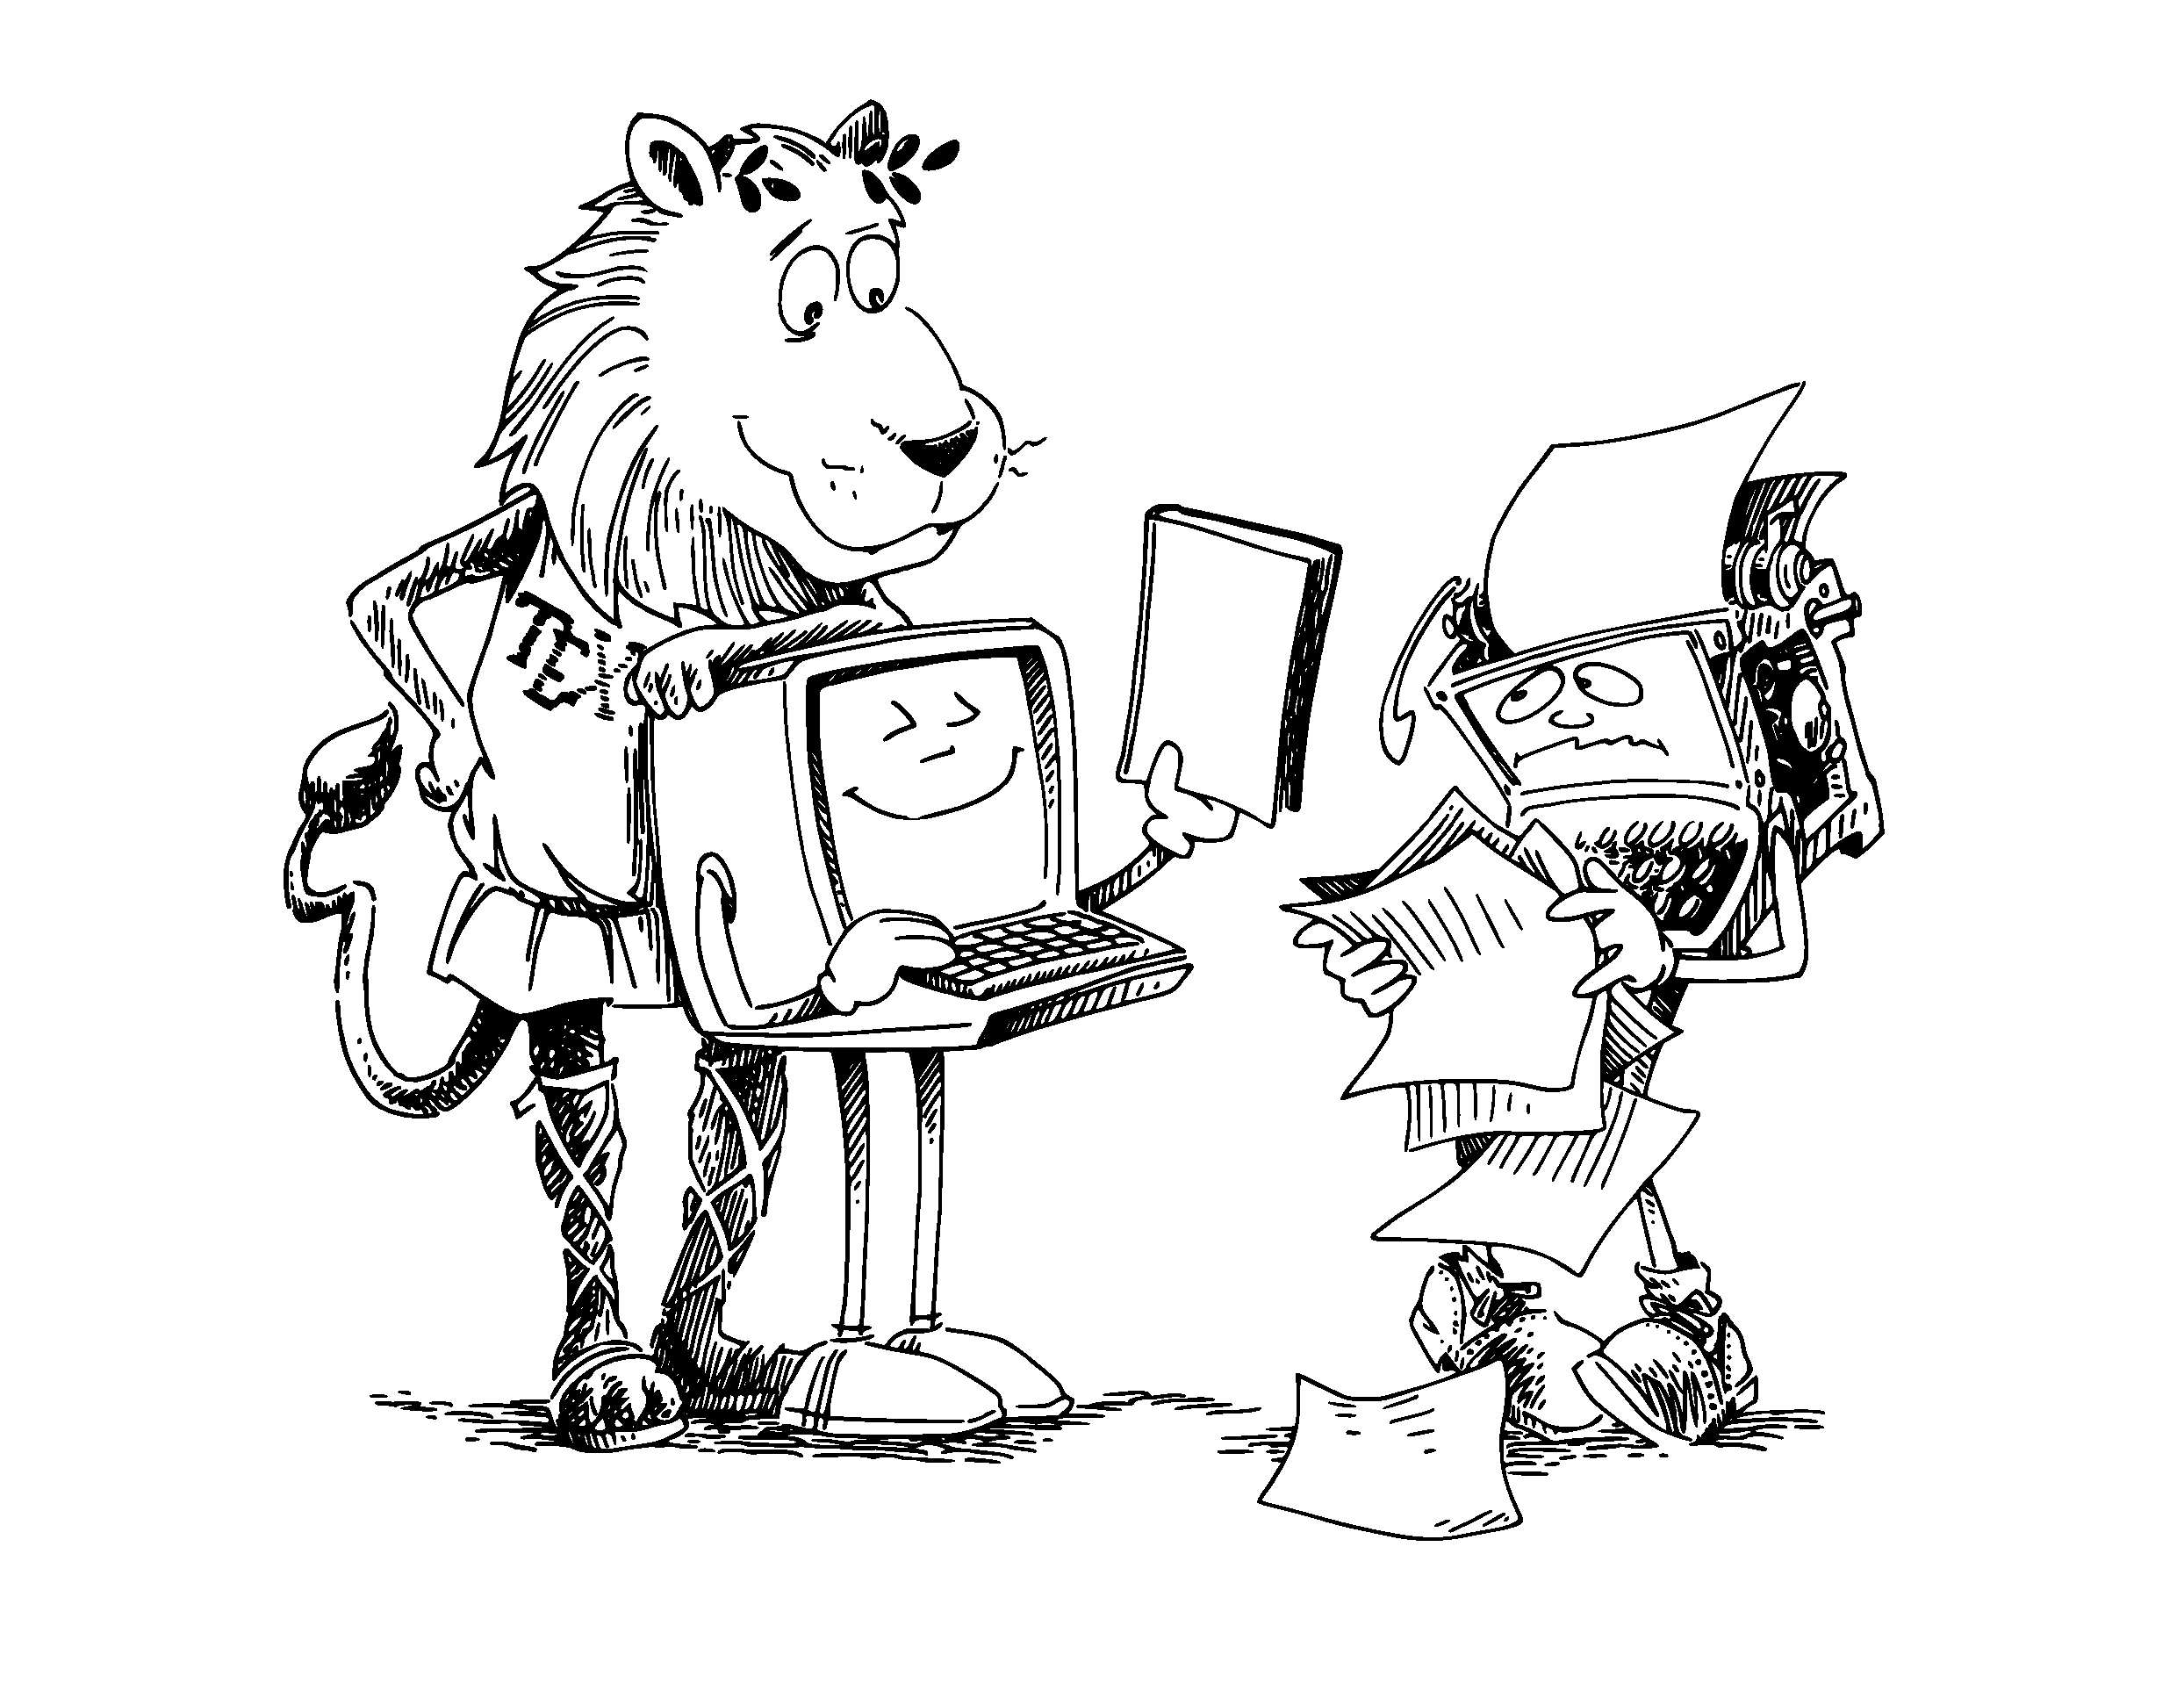
\includegraphics[width=.3\textwidth]{Ch2}
\bicaption{单幅图}{single image}\label{fig:1}
\end{figure}
\begin{lstlisting}[language=TeX]
\begin{figure}[H]%可选htbp
	\centering
	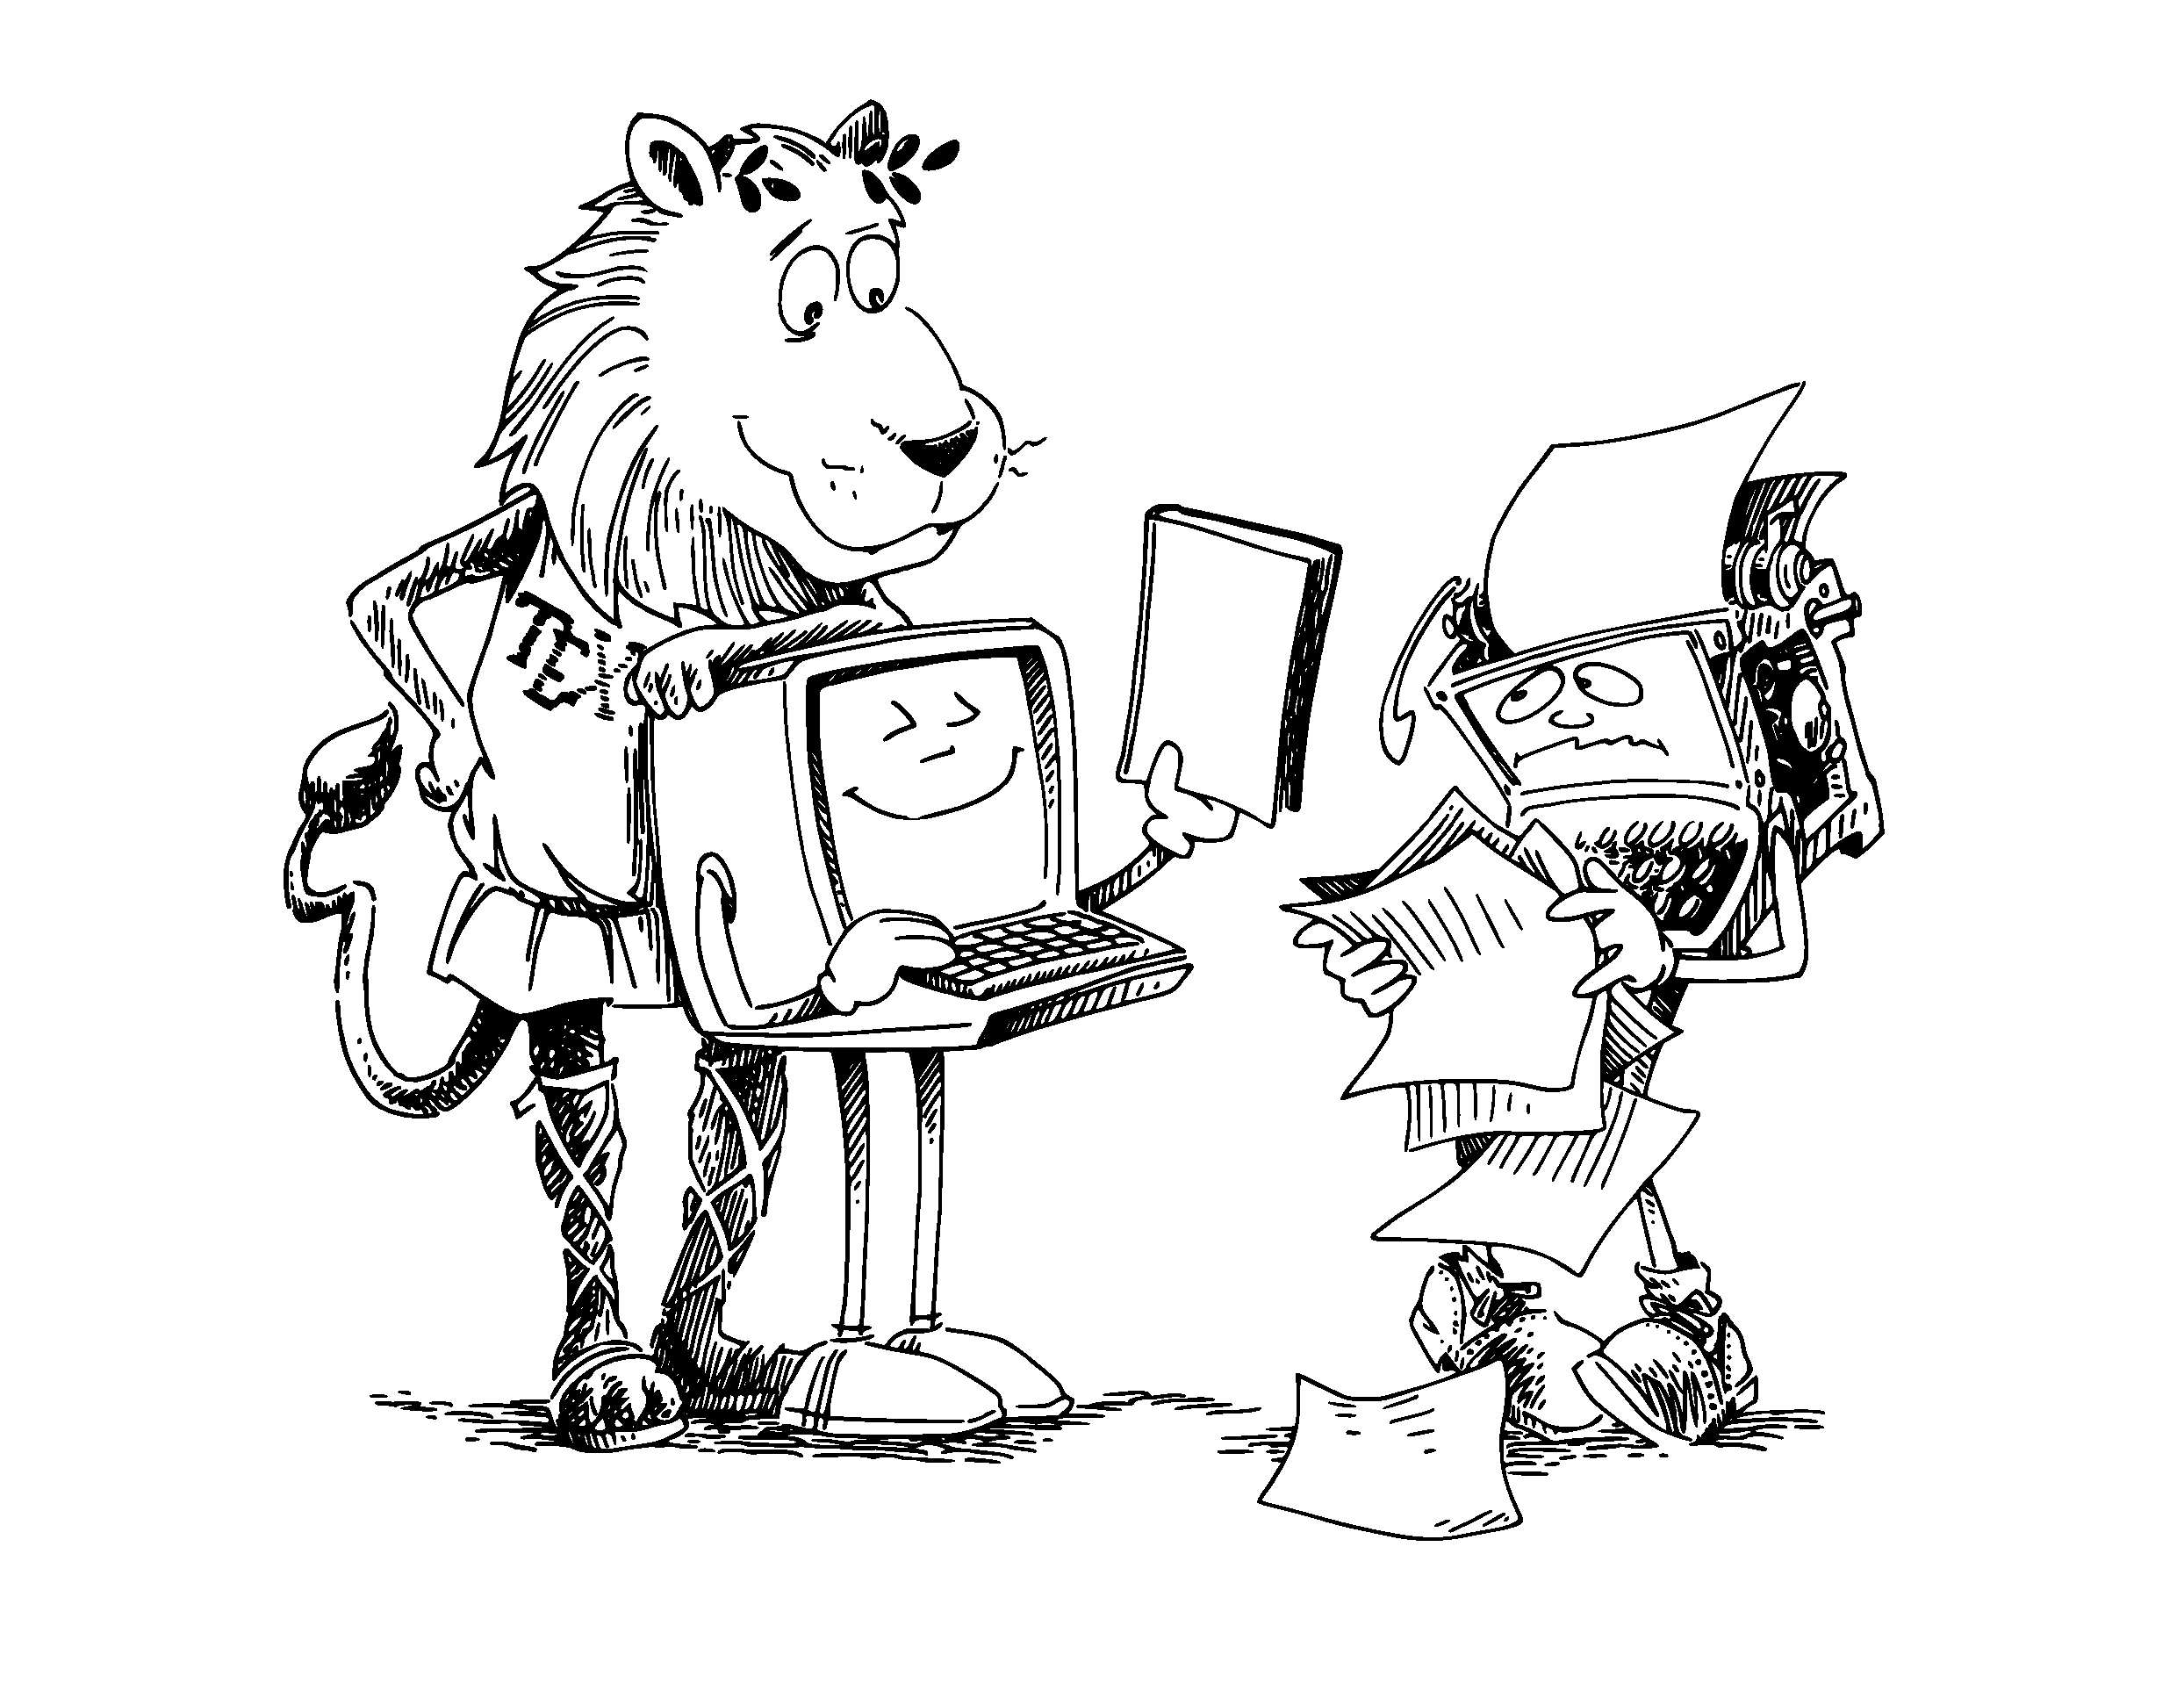
\includegraphics[width=.3\textwidth]{Ch2}
	\bicaption{单幅图}{single image}\label{fig:1}
\end{figure}
\end{lstlisting}

图片与表格可选参数

\begin{itemize}
	\item H 就在当前位置不动。
	\item h 当前位置。将图形放置在正文文本中给出该图形环境的地方。如果本页所剩的页面不够,这一参数将不起作用。
	\item t 顶部。将图形放置在页面的顶部。
	\item b 底部。将图形放置在页面的底部。
	\item p 浮动页。将图形放置在一只允许有浮动对象的页面上。
\end{itemize}

\subsection{多图带子标题+长标题}
\begin{figure}[htp]
	\begin{subfigure}[b]{0.3\textwidth}
		\centering
		\includegraphics[width=\textwidth]{example-image}
		\bisubcaption{中文标题}{English title}\label{fig:2-1}
	\end{subfigure}
	\hfill
	\begin{subfigure}[b]{0.3\textwidth}
		\centering
		\includegraphics[width=\textwidth]{example-image}
		\bisubcaption{中文标题}{English title}\label{fig:2-2}
	\end{subfigure}
	\hfill
	\begin{subfigure}[b]{0.3\textwidth}
		\centering
		\includegraphics[width=\textwidth]{example-image}
		\bisubcaption{中文标题}{English title}\label{fig:2-3}
	\end{subfigure}
	\bicaption{第二个图名字第二个图名字第二个图名字第二个图名字第二个图名字第二个图名字第二个图名字第二个图名字第二个图名字第二个图名字}{English title}\label{fig:2}
\end{figure}
\vspace{.5cm}

\begin{lstlisting}[language=TeX]
\begin{figure}[htp]
	\begin{subfigure}[b]{0.3\textwidth}
		\centering
		\includegraphics[width=\textwidth]{example-image}
		\bisubcaption{中文标题}{English title}\label{fig:2-1}
	\end{subfigure}
	\hfill
	\begin{subfigure}[b]{0.3\textwidth}
		\centering
		\includegraphics[width=\textwidth]{example-image}
		\bisubcaption{中文标题}{English title}\label{fig:2-2}
	\end{subfigure}
	\hfill
	\begin{subfigure}[b]{0.3\textwidth}
		\centering
		\includegraphics[width=\textwidth]{example-image}
		\bisubcaption{中文标题}{English title}\label{fig:2-3}
	\end{subfigure}
	\bicaption{第二个图名字第二个图名字第二个图名字第二个图名字第二个图名字第二个图名字第二个图名字第二个图名字第二个图名字第二个图名字}{English title}\label{fig:2}
\end{figure}
\end{lstlisting}

\subsection{图引用}
引用: 图\ref{fig:1}。

引用图 2 的第 1 个子图:\ref{fig:2-1}。
 
引用图 2 的第 1-3 个子图 \cref{fig:2-1} -\subref{fig:2-3}。

\begin{lstlisting}
引用: 图\ref{fig:1}。引用图 2 的第 1 个子图:\ref{fig:2-1}。引用图 2 的第 1-3 个子图 \cref{fig:2-1} -\subref{fig:2-3}。
\end{lstlisting}
使用\myverb{\cref{}}命令在引用时不需要额外加“图”。例如 :

\cref{fig:2-1}

\begin{lstlisting}
\cref{fig:2-1}
\end{lstlisting}

\section{表}
表格制作工具\footnote{推荐俩个表格工具或网站\begin{itemize}
		\item \textbf{\href{www.tablesgenerator.com}{在线表格生成}\;:}在线编辑表格并转化为\LaTeX 代码
		\item \textbf{\href{https://www.ctan.org/tex-archive/support/excel2latex/}{Excel 2\LaTeX}\;:
		}Excel插件,可以将Excel表格转化为\LaTeX 代码
\end{itemize}}。
\subsection{三线表}
\begin{table}[H]
	\centering
	\bicaption{第一个表名字}{English title}\label{tab:1}
	\begin{tabular}{ccc}
		\toprule
		呵&呵呵&呵呵呵\\
		\midrule
		1&    &   \\
		2&    &   \\
		\bottomrule
	\end{tabular}
\end{table}
\begin{lstlisting}[language=TeX]
\begin{table}[H]
	\centering
	\bicaption{第一个表名字}{English title}\label{tab:1}
	\begin{tabular}{ccc}
		\toprule
		呵&呵呵&呵呵呵\\
		\midrule
		1&    &   \\
		2&    &   \\
		\bottomrule
	\end{tabular}
\end{table}
\end{lstlisting}

\subsection{单元格合并}
\begin{table}[H]
\centering
\bicaption{单元格合并演示}{Cell merge demonstration}\label{tab:hebing}
\begin{tabular}{cccccc}
	\toprule
	国家或地区             & \multicolumn{5}{c}{数据}\\
	\midrule
	\multirow{4}*{意大利}  &  \multirow{2}*{累计确诊}  & LSTM  & 789479.9582  & 0.99762  & 7.6276\% \\
	
	~                     &  ~                         &  BP & 1400034.6229 & 0.80102 & 15.331\%\\
	\Xcline{2-6}{0.5pt}
	~                     &  \multirow{2}*{累计死亡}   &  LSTM & 3156.1792 & 0.99843 & 2.2079\% \\
	
	~                     &  ~                         & BP &  5650.3914 & 0.99886 & 4.1139\% \\
	\toprule
\end{tabular}
\end{table}
\begin{lstlisting}[language=TeX]	
\begin{table}[H]
	\centering
	\bicaption{单元格合并演示}{Cell merge demonstration}\label{tab:hebing}
	\begin{tabular}{cccccc}
		\toprule
		国家或地区             & \multicolumn{5}{c}{数据}\\
		\midrule
		\multirow{4}*{意大利}  &  \multirow{2}*{累计确诊}  & LSTM  & 789479.9582  & 0.99762  & 7.6276\% \\
		
		~                     &  ~                         &  BP & 1400034.6229 & 0.80102 & 15.331\%\\
		\Xcline{2-6}{0.5pt}
		~                     &  \multirow{2}*{累计死亡}   &  LSTM & 3156.1792 & 0.99843 & 2.2079\% \\
		
		~                     &  ~                         & BP &  5650.3914 & 0.99886 & 4.1139\% \\
		
		\midrule
		\multirow{4}*{丹麦}   &  \multirow{2}*{累计确诊}  & LSTM & 131857.386  & 0.93468 & 6.6074\% \\
		
		~                     &  ~                       &  BP  & 293525.3201 & 0.79159  & 17.629\%\\
		\Xcline{2-6}{0.5pt}
		~                     &  \multirow{2}*{累计死亡}  &  LSTM & 75.4425& 0.99751 & 2.3149 \%\\
		
		~                     &  ~                       &   BP  & 206.0897  & 0.99902  & 7.0008\% \\
		\toprule
	\end{tabular}
\end{table}
\end{lstlisting}
\subsection{带注释表}

\begin{table}[H]
	\centering
	\bicaption{带注释表}{English title}\label{tab:2}
	\begin{threeparttable}
		\begin{tabular}{cccccc}
			\toprule
			国家或地区             & \multicolumn{5}{c}{数据}\\
			\midrule
			\multirow{4}*{意大利}  &  \multirow{2}*{累计确诊}  & LSTM  & 789479.9582  & 0.99762  & 7.6276\% \\
			
			~                     &  ~                         &  BP & 1400034.6229 & 0.80102 & 15.331\%\\
			\Xcline{2-6}{0.5pt}
			~                     &  \multirow{2}*{累计死亡}   &  LSTM & 3156.1792 & 0.99843 & 2.2079\% \\
			
			~                     &  ~                         & BP &  5650.3914 & 0.99886 & 4.1139\% \\
			\toprule
		\end{tabular}
		\begin{tablenotes}
			\footnotesize
			\item S: single damage; R: repetitive damage; M: multiple damage
		\end{tablenotes}
	\end{threeparttable}
\end{table}


\begin{lstlisting}[language=TeX]
\begin{table}[H]
	\centering
	\bicaption{带注释表}{English title}\label{tab:2}
	\begin{threeparttable}
		\begin{tabular}{cccccc}
			\toprule
			国家或地区             & \multicolumn{5}{c}{数据}\\
			\midrule
			\multirow{4}*{意大利}  &  \multirow{2}*{累计确诊}  & LSTM  & 789479.9582  & 0.99762  & 7.6276\% \\
			
			~                     &  ~                         &  BP & 1400034.6229 & 0.80102 & 15.331\%\\
			\Xcline{2-6}{0.5pt}
			~                     &  \multirow{2}*{累计死亡}   &  LSTM & 3156.1792 & 0.99843 & 2.2079\% \\
			
			~                     &  ~                         & BP &  5650.3914 & 0.99886 & 4.1139\% \\
			\toprule
		\end{tabular}
		\begin{tablenotes}
			\footnotesize
			\item S: single damage; R: repetitive damage; M: multiple damage
		\end{tablenotes}
	\end{threeparttable}
\end{table}
\end{lstlisting}
\subsection{跨页长表格}
\begin{center}
\setlength{\tabcolsep}{10mm}
\begin{longtable}{ccc}
	\bicaption{符号含义}{Symbolic Meaning}\label{tab:long}\\
	\endfirsthead
 	\multicolumn{3}{c}{\makecell{\zihao{5}\kaishu 表~\thetable 符号含义(续)\vspace{-8pt}\\\zihao{5}\kaishu Table\;\thetable \;Symbolic Meaning(continue)}}\\
	\toprule
	符号      &   表示含义              &     单位 \\
	\toprule
	\endhead
	\toprule
	符号      &   表示含义              &     单位 \\
	\toprule
	$t$      & 时间                   &     $s$\\
	\midrule
	...     &  ...                   &    ...\\
	\midrule 
	...    &  ...                   &    ...\\
	\midrule 
	...     &  ...                  &    ...\\
	\midrule
	...     &  ...                   &    ...\\
	\midrule 
	...    &  ...                   &    ...\\
	\midrule 
	...     &  ...                  &    ...\\ 
	\midrule
	...     &  ...                   &    ...\\
	\midrule 
	...    &  ...                   &    ...\\
	\midrule
	...     &  ...                   &    ...\\
	\midrule 
	...    &  ...                   &    ...\\
	\midrule 
	...     &  ...                  &    ...\\
	\midrule
	...     &  ...                   &    ...\\
	\midrule 
	...    &  ...                   &    ...\\
	\midrule 
	...     &  ...                  &    ...\\ 
	\midrule
	...     &  ...                   &    ...\\
	\midrule 
	...    &  ...                   &    ...\\
	\midrule
	...     &  ...                   &    ...\\
	\midrule 
	...    &  ...                   &    ...\\
	\midrule 
	...     &  ...                  &    ...\\
	\midrule
	...     &  ...                   &    ...\\
	\midrule 
	...    &  ...                   &    ...\\
	\midrule 
	...     &  ...                  &    ...\\ 
	\midrule
	...     &  ...                   &    ...\\
	\midrule 
	...    &  ...                   &    ...\\
	\midrule
	...     &  ...                   &    ...\\
	\midrule 
	...    &  ...                   &    ...\\
	\midrule 
	...     &  ...                  &    ...\\
	\midrule
	...     &  ...                   &    ...\\
	\midrule 
	...    &  ...                   &    ...\\
	\midrule 
	...     &  ...                  &    ...\\ 
	\midrule
	...     &  ...                   &    ...\\
	\midrule 
	...    &  ...                   &    ...\\
	\bottomrule
\end{longtable}
\end{center}

\begin{lstlisting}[language=TeX]
\begin{center}
	\setlength{\tabcolsep}{10mm}
	\begin{longtable}{ccc}
		\bicaption{符号含义}{Symbolic Meaning}\label{tab:2}\\
		\endfirsthead
		\multicolumn{3}{c}{\makecell{\zihao{5}\kaishu 表~\thetable 符号含义(续)\vspace{-8pt}\\\zihao{5}\kaishu Table\;\thetable \;Symbolic Meaning(continue)}}\\
		\toprule
		符号      &   表示含义              &     单位 \\
		\toprule
		\endhead
		\toprule
		符号      &   表示含义              &     单位 \\
		\toprule
		$t$      & 时间                   &     $s$\\
		\midrule
		...     &  ...                   &    ...\\
		\midrule 
		...    &  ...                   &    ...\\
		\midrule 
		...     &  ...                  &    ...\\
		\midrule
		省略部分
		\bottomrule
	\end{longtable}
\end{center}
\end{lstlisting}

\subsection{表格引用}
引用: 表\ref{tab:1}。 引用表:\ref{tab:hebing}。 引用:表\ref{tab:long}。
\begin{lstlisting}
引用: 图\ref{tab:1}。 引用图 2 的第一个子图:\ref{tab:hebing}。 引用: 图 \ref{fig:long}。
\end{lstlisting}

使用\myverb{\cref{}}命令在引用时不需要额外加“表”。例如 :

\cref{tab:hebing}

\begin{lstlisting}
	\cref{tab:hebing}
\end{lstlisting}


\section{数学环境}
\subsection{定理引理证明}
\begin{theorem}
这是一个定理
\end{theorem}
\begin{lemma}
这是一个引理
\end{lemma}
\begin{proof}
这是一个证明
\end{proof}
\begin{lstlisting}[language=TeX]
\begin{theorem}
	这是一个定理
\end{theorem}
\begin{lemma}
	这是一个引理
\end{lemma}
\begin{proof}
	这是一个证明
\end{proof}
\end{lstlisting}

\subsection{数学公式}
\begin{align*}
	x &= t + \cos t +1 \\
	y &= 2 \sin t
\end{align*}
\begin{align}
	x &= t + \cos t +1 \\
	y &= 2 \sin t
\end{align}
\begin{equation}\label{equ:1}
	\begin{split}
		\cos 2x &= \cos^2 x -\sin^2 x \\
		&= 2 \cos^2 x -1
	\end{split}
\end{equation}
\begin{equation*}
	\cos 2x = \cos^2 x -\sin^2 x 
\end{equation*}
\[ \cos 2x = \cos^2 x -\sin^2 x \]
\begin{equation}
D(x)= \begin{cases}
		1, & \text{如果} x \in \mathbb{Q}; \\
		0, & \text{如果} x \in \mathbb{R} \setminus \mathbb{Q}.
	\end{cases}
\end{equation}
\begin{lstlisting}[language=TeX]
\begin{align*}
	x &= t + \cos t +1 \\
	y &= 2 \sin t
\end{align*}
\begin{align}
	x &= t + \cos t +1 \\
	y &= 2 \sin t
\end{align}
\begin{equation}
	\begin{split}
		\cos 2x &= \cos^2 x -\sin^2 x \\
		&= 2 \cos^2 x -1
	\end{split}
\end{equation}
\begin{equation*}
	\cos 2x = \cos^2 x -\sin^2 x 
\end{equation*}
\[ \cos 2x = \cos^2 x -\sin^2 x \]
\begin{equation}
	D(x)= \begin{cases}
		1, & \text{如果} x \in \mathbb{Q}; \\
		0, & \text{如果} x \in \mathbb{R} \setminus \mathbb{Q}.
	\end{cases}
\end{equation}
\end{lstlisting}

\subsection{公式引用}
引用: 公式 (\ref{equ:1}), 公式 \eqref{equ:1}
\begin{lstlisting}
引用: 公式 (\ref{equ:1}), 公式 \eqref{equ:1}
\end{lstlisting}

使用\myverb{\cref{}}命令在引用时不需要额外加“公式”和“( )”。例如 :

\cref{equ:1}

\begin{lstlisting}
	\cref{equ:1}
\end{lstlisting}


\section{参考文献}
参考文献建议使用\myverb{bibtex},若你想使用列表方法,自行百度。

单个引用\cite{choudhary2023multi}。连续引用\cite{kumar2020improved,zhu2019deformable}。连续引用\cite{choudhary2023multi,zhu2019deformable,ZDGC202202020,JXXB201907002}
\begin{lstlisting}
单个引用\cite{choudhary2023multi}。连续引用\cite{kumar2020improved,zhu2019deformab
	le}。连续引用\cite{choudhary2023multi,zhu2019deformable,ZDGC202202020,JXXB201907
	002}
\end{lstlisting}
生成文献 Bib\TeX 引用格式可以使用谷歌学术。知网在生成文献 Bib\TeX 引用格式需要点很多次,因此找朋友开发了一个油猴插件,可以直接复制知网文献的Bib\TeX 格式。

插件地址:\begin{itemize}
	\item 游猴 :\href{https://greasyfork.org/zh-CN/scripts/444428}{ \;\;https://greasyfork.org/zh-CN/scripts/444428}

	\item GitHub \faGithub :\href{https://github.com/BNDou/getCnkiLiteratureBibTex}{ \;\;https://github.com/BNDou/getCnkiLiteratureBibTex}
\end{itemize}

\section{列表}


\subsection{有序列表}
\begin{minipage}[t]{0.48\textwidth}
	\begin{lstlisting}[language=TeX]
		\begin{enumerate}
			\item 
			\item 
			\item 
		\end{enumerate}
	\end{lstlisting} 
\end{minipage}
\begin{minipage}[t]{0.48\textwidth}
	\rule[-10pt]{10cm}{0em}
	\begin{enumerate}
		\item 
		\item 
		\item 
	\end{enumerate}
\end{minipage}
\subsection{无序列表}
\begin{minipage}[t]{0.48\textwidth}
	\begin{lstlisting}[language=TeX]
		\begin{itemize}
			\item 
			\item 
			\item 
		\end{itemize}
	\end{lstlisting} 
\end{minipage}
\begin{minipage}[t]{0.48\textwidth}
	\rule[-10pt]{10cm}{0em}
	\begin{itemize}
		\item 
		\item 
		\item 
	\end{itemize}
\end{minipage}

\section{化学方程式}
考虑到一些同学需要写化学公式,本模板加载了宏包  \myverb{mhchem} 和 \myverb{chemfig}。 

化学方程式直用\myverb{mhchem}宏包提供的以下代码即可。
\begin{lstlisting}
	\ce{...}
\end{lstlisting} 
\begin{center}
	\ce{Zn^2+  <=>[+ 2OH-][+ 2H+]  $\underset{\text{这是沉淀}}{\ce{Zn(OH)2 v}}$  <=>[+ 2OH-][+ 2H+]  $\underset{\text{这是离子}}{\ce{[Zn(OH)4]^2-}}$}
\end{center}
结构式用\myverb{chemfig}宏包提供的功能。
\begin{center}
	\chemfig{[:-30]HO--[:30](<[2]OH)-(<:[6]OH)
		-[:30](<:[2]OH)-(<:[6]OH)-[:30](=[2]O)-H}
\end{center}

\section{生僻字}
引用过程中可能出现某人姓名中有生僻字导致生成的PDF中无法显示这个字,给出一个最简单的解决方案:将生僻字自己截图,然后插入文中。

eg:{\lower0.4ex\hbox{
\includegraphics[width=1.1em]{huaji}}}是我造的一个字
\begin{lstlisting}[language=TeX]
	eg:{\lower0.4ex\hbox{
\includegraphics[width=1.1em]{huaji}}}是我造的一个字
\end{lstlisting}
\bibliography{chapter/10references.bib}%参考文献
%% !TEX root = main.tex
\begin{appendix}

\chapter{论文无需附录去掉该部分}
\section{测试}
\subsection{图}
\begin{figure}[H]
	\centering
	\includegraphics[scale=0.5]{example-image}
	\caption{长标题测试。这是个很长很长很长很长很长很长很长很长很长很长很长很长很长很长很长很长很长很长很长的标题}
\end{figure}
\section{冒泡排序算法}
\begin{lstlisting}[language=Java]
	/*冒泡排序算法*/ 
	public static void bubble_sort(int[] arr) {
		int i, j, temp, len = arr.length;
		for (i = 0; i < len - 1; i++)
		for (j = 0; j < len - 1 - i; j++) 
		if (arr[j] > arr[j + 1]) {
			temp = arr[j];
			arr[j] = arr[j + 1];
			arr[j + 1] = temp;
		}
	}
\end{lstlisting}



\end{appendix}% 附录
% ---------- 后文 --------- %
\backmatter
% !TEX root = main.tex
\begin{achievement}
\begin{enumerate}[font=\heiti]
\item[一、] {\heiti 学术论文}
\begin{enumerate}[{[}1{]},parsep=-.1cm]
	\item {\heiti 章安良}, 刘尉悦, 蒋志迪, 费景臣. 基于声表面波技术的数字微流体微加热器研究[J]. 微纳电子技术, 2008, 45(7): 411-414.(对应论文第3章)
	\item {\heiti Yan Liu}, Chenxiang Lin, Hanying Li, Hao Yan. Protein nanoarrays: Aptamer-directed self-assembly of protein arrays on a DNA nanostructure[J]. Angew Chem Int Ed, 2005, 44(25): 4333-4338.(SCI一区, 对应论文第4章)
\end{enumerate}

\item[二、] {\heiti 国家发明专利}
\begin{enumerate}[{[}1{]},parsep=-.1cm]
	\item {\heiti XXX}, XXX, XXX, XXX. 专利题目. 专利类型. 授权公告号, 授权公告日
	\item XXX, XXX, XXX, XXX. 专利题目. 专利类型. 申请公布号, 申请公布日.
	\item {\heiti 张凯军}, 赵永杰, 陈朝岗. 轨道火车及高速轨道火车紧急安全制动辅助装置. 实用新型专利. CN201220158825.2. 2012-04-05.
\end{enumerate}

\item[三、] {\heiti 科研项目}
\begin{enumerate}[{[}1{]},parsep=-.1cm]
	\item 项目类型, 项目名称, 项目编号, 资助单位, 起止时间, 主持/参与.
\end{enumerate}

\item[四、] {\heiti 其他}
\begin{enumerate}[{[}1{]},parsep=-.1cm]
	\item 
\end{enumerate}

\end{enumerate}
\end{achievement}%学术成果
% !TEX root = main.tex
\begin{ack}
关山难越,谁悲失路之人;萍水相逢,尽是他乡之客。

愿你毕业顺利!



\end{ack}%致谢
\end{document}
\end{lstlisting}
\section{文件夹组成}
文件夹组成如下:

\begin{forest}
	pic dir tree,
	where level=0{}{directory,
	},
	[文件夹
	[chapter
	[01coverinfor.tex {\color{gray}论文封面信息},file2
	]
	[02abstract.tex {\color{gray}中英文摘要},file2
	]
	[03denotation.tex {\color{gray}主要符号对照表(可取消)},file2
	]
	[04chapter1.tex {\color{gray}第一章},file2
	]
	[10references.tex {\color{gray}参考文献},file2
	]
	[11appendices.tex {\color{gray}附录(可取消)},file2
	]
	[12achievement.tex {\color{gray}攻读学位期间取得的学术成果},file2
	]
	[13acknowledgement.tex {\color{gray}致谢},file2
	]
	]
	[figure
	[logo {\color{gray}封面logo}
	]
	[page2.png {\color{gray}论文图片存放}, file
	]
	[..., file
	]
	]
	[main.tex {\color{gray}主文件},file2
	]
	[TYUSTthesis.cls {\color{gray}模板格式文件},file2
	]
	]
\end{forest}

\section{参数说明}
本文档结合了硕士与博士学位论文模板,因此在加载TYUSTthesis文档类时有三个可选参数:
\begin{itemize}
	\item master 硕士学位论文(default)
	\item doctor 博士学位论文
	\item encover 博士学位论文英文封面
	\item declare 学位论文原创说明与授权说明
\end{itemize}

例如你想使用硕士论文并包含授权页,可使用下边命令
\begin{lstlisting}
\documentclass[master,declare]{TYUSTthesis}
\end{lstlisting}

你想使用博士论文并包含英文封面,可使用下边命令
\begin{lstlisting}
\documentclass[doctor,encover]{TYUSTthesis}
\end{lstlisting}

你想使用博士论文,包含英文封面,包含授权页,可使用下边命令
\begin{lstlisting}
\documentclass[doctor,encover,declare]{TYUSTthesis}
\end{lstlisting}

\section{预加载宏包}
\begin{table}[hp]
	\renewcommand\arraystretch{1.2}
	\centering  % 显示位置为中间
	\bicaption{预加载宏包}{Preloaded macro package}\label{tab:1}
	\begin{tabular}{ll||ll} %第一列设置宽度为45pt 全为左对齐 没有分割线
		\hline
		宏包 		&说明		    & 宏包 	   & 说明     \\
		\hline 
		geometry  &页边距	     &gbt7714	  &参考文献格式 \\
		float	  &浮动体	     &setspace	  & 设置间距  \\
		mwe 	  &提供示例图片  & graphicx  & 插图       \\
		booktabs  &三线表       & longtable &长表格      \\
		threeparttable&注释表&makecell   &表格内容换行 \\
		multirow  & 合并单元格& calc      & 距离计算   \\
		fontawesome& 字体 &listings    & 代码环境         \\
		mhchem     &化学环境     &chemfig   &化学环境     \\
		amsmath    &数学环境    &amsthm     &数学环境     \\
		amssymb    &数学环境    &amsfonts   &数学环境     \\
		hyperref   & 超链接    &enumitem    &列表         \\
		cleveref   & 引用格式   & algorithm2e & 算法\\
		titletoc   & 目录设置  &setspace     &设置间距    \\
		caption    & 图表标题  &tikz        &画图         \\
		subcaption & 图表标题  &tcolorbox   & 彩色盒子   \\
		bicaption &  图表标题   & xparse    &  边注       \\
		marginnote&  边注      &forest      &             \\
		zhlipsum    &            &needspace  &               \\
        lipsum     &    & &\\
		\hline
	\end{tabular}
\end{table}
